% Generated by Sphinx.
\def\sphinxdocclass{report}
\documentclass[letterpaper,10pt,english]{sphinxmanual}
\usepackage[utf8]{inputenc}
\DeclareUnicodeCharacter{00A0}{\nobreakspace}
\usepackage[T1]{fontenc}
\usepackage{babel}
\usepackage{times}
\usepackage[Bjarne]{fncychap}
\usepackage{longtable}
\usepackage{sphinx}


\title{CS6795 Labs and Assignments Documentation}
\date{October 03, 2011}
\release{1.0}
\author{Reuben Peter-Paul}
\newcommand{\sphinxlogo}{}
\renewcommand{\releasename}{Release}
\makeindex

\makeatletter
\def\PYG@reset{\let\PYG@it=\relax \let\PYG@bf=\relax%
    \let\PYG@ul=\relax \let\PYG@tc=\relax%
    \let\PYG@bc=\relax \let\PYG@ff=\relax}
\def\PYG@tok#1{\csname PYG@tok@#1\endcsname}
\def\PYG@toks#1+{\ifx\relax#1\empty\else%
    \PYG@tok{#1}\expandafter\PYG@toks\fi}
\def\PYG@do#1{\PYG@bc{\PYG@tc{\PYG@ul{%
    \PYG@it{\PYG@bf{\PYG@ff{#1}}}}}}}
\def\PYG#1#2{\PYG@reset\PYG@toks#1+\relax+\PYG@do{#2}}

\def\PYG@tok@gd{\def\PYG@tc##1{\textcolor[rgb]{0.63,0.00,0.00}{##1}}}
\def\PYG@tok@gu{\let\PYG@bf=\textbf\def\PYG@tc##1{\textcolor[rgb]{0.50,0.00,0.50}{##1}}}
\def\PYG@tok@gt{\def\PYG@tc##1{\textcolor[rgb]{0.00,0.25,0.82}{##1}}}
\def\PYG@tok@gs{\let\PYG@bf=\textbf}
\def\PYG@tok@gr{\def\PYG@tc##1{\textcolor[rgb]{1.00,0.00,0.00}{##1}}}
\def\PYG@tok@cm{\let\PYG@it=\textit\def\PYG@tc##1{\textcolor[rgb]{0.25,0.50,0.56}{##1}}}
\def\PYG@tok@vg{\def\PYG@tc##1{\textcolor[rgb]{0.73,0.38,0.84}{##1}}}
\def\PYG@tok@m{\def\PYG@tc##1{\textcolor[rgb]{0.13,0.50,0.31}{##1}}}
\def\PYG@tok@mh{\def\PYG@tc##1{\textcolor[rgb]{0.13,0.50,0.31}{##1}}}
\def\PYG@tok@cs{\def\PYG@tc##1{\textcolor[rgb]{0.25,0.50,0.56}{##1}}\def\PYG@bc##1{\colorbox[rgb]{1.00,0.94,0.94}{##1}}}
\def\PYG@tok@ge{\let\PYG@it=\textit}
\def\PYG@tok@vc{\def\PYG@tc##1{\textcolor[rgb]{0.73,0.38,0.84}{##1}}}
\def\PYG@tok@il{\def\PYG@tc##1{\textcolor[rgb]{0.13,0.50,0.31}{##1}}}
\def\PYG@tok@go{\def\PYG@tc##1{\textcolor[rgb]{0.19,0.19,0.19}{##1}}}
\def\PYG@tok@cp{\def\PYG@tc##1{\textcolor[rgb]{0.00,0.44,0.13}{##1}}}
\def\PYG@tok@gi{\def\PYG@tc##1{\textcolor[rgb]{0.00,0.63,0.00}{##1}}}
\def\PYG@tok@gh{\let\PYG@bf=\textbf\def\PYG@tc##1{\textcolor[rgb]{0.00,0.00,0.50}{##1}}}
\def\PYG@tok@ni{\let\PYG@bf=\textbf\def\PYG@tc##1{\textcolor[rgb]{0.84,0.33,0.22}{##1}}}
\def\PYG@tok@nl{\let\PYG@bf=\textbf\def\PYG@tc##1{\textcolor[rgb]{0.00,0.13,0.44}{##1}}}
\def\PYG@tok@nn{\let\PYG@bf=\textbf\def\PYG@tc##1{\textcolor[rgb]{0.05,0.52,0.71}{##1}}}
\def\PYG@tok@no{\def\PYG@tc##1{\textcolor[rgb]{0.38,0.68,0.84}{##1}}}
\def\PYG@tok@na{\def\PYG@tc##1{\textcolor[rgb]{0.25,0.44,0.63}{##1}}}
\def\PYG@tok@nb{\def\PYG@tc##1{\textcolor[rgb]{0.00,0.44,0.13}{##1}}}
\def\PYG@tok@nc{\let\PYG@bf=\textbf\def\PYG@tc##1{\textcolor[rgb]{0.05,0.52,0.71}{##1}}}
\def\PYG@tok@nd{\let\PYG@bf=\textbf\def\PYG@tc##1{\textcolor[rgb]{0.33,0.33,0.33}{##1}}}
\def\PYG@tok@ne{\def\PYG@tc##1{\textcolor[rgb]{0.00,0.44,0.13}{##1}}}
\def\PYG@tok@nf{\def\PYG@tc##1{\textcolor[rgb]{0.02,0.16,0.49}{##1}}}
\def\PYG@tok@si{\let\PYG@it=\textit\def\PYG@tc##1{\textcolor[rgb]{0.44,0.63,0.82}{##1}}}
\def\PYG@tok@s2{\def\PYG@tc##1{\textcolor[rgb]{0.25,0.44,0.63}{##1}}}
\def\PYG@tok@vi{\def\PYG@tc##1{\textcolor[rgb]{0.73,0.38,0.84}{##1}}}
\def\PYG@tok@nt{\let\PYG@bf=\textbf\def\PYG@tc##1{\textcolor[rgb]{0.02,0.16,0.45}{##1}}}
\def\PYG@tok@nv{\def\PYG@tc##1{\textcolor[rgb]{0.73,0.38,0.84}{##1}}}
\def\PYG@tok@s1{\def\PYG@tc##1{\textcolor[rgb]{0.25,0.44,0.63}{##1}}}
\def\PYG@tok@gp{\let\PYG@bf=\textbf\def\PYG@tc##1{\textcolor[rgb]{0.78,0.36,0.04}{##1}}}
\def\PYG@tok@sh{\def\PYG@tc##1{\textcolor[rgb]{0.25,0.44,0.63}{##1}}}
\def\PYG@tok@ow{\let\PYG@bf=\textbf\def\PYG@tc##1{\textcolor[rgb]{0.00,0.44,0.13}{##1}}}
\def\PYG@tok@sx{\def\PYG@tc##1{\textcolor[rgb]{0.78,0.36,0.04}{##1}}}
\def\PYG@tok@bp{\def\PYG@tc##1{\textcolor[rgb]{0.00,0.44,0.13}{##1}}}
\def\PYG@tok@c1{\let\PYG@it=\textit\def\PYG@tc##1{\textcolor[rgb]{0.25,0.50,0.56}{##1}}}
\def\PYG@tok@kc{\let\PYG@bf=\textbf\def\PYG@tc##1{\textcolor[rgb]{0.00,0.44,0.13}{##1}}}
\def\PYG@tok@c{\let\PYG@it=\textit\def\PYG@tc##1{\textcolor[rgb]{0.25,0.50,0.56}{##1}}}
\def\PYG@tok@mf{\def\PYG@tc##1{\textcolor[rgb]{0.13,0.50,0.31}{##1}}}
\def\PYG@tok@err{\def\PYG@bc##1{\fcolorbox[rgb]{1.00,0.00,0.00}{1,1,1}{##1}}}
\def\PYG@tok@kd{\let\PYG@bf=\textbf\def\PYG@tc##1{\textcolor[rgb]{0.00,0.44,0.13}{##1}}}
\def\PYG@tok@ss{\def\PYG@tc##1{\textcolor[rgb]{0.32,0.47,0.09}{##1}}}
\def\PYG@tok@sr{\def\PYG@tc##1{\textcolor[rgb]{0.14,0.33,0.53}{##1}}}
\def\PYG@tok@mo{\def\PYG@tc##1{\textcolor[rgb]{0.13,0.50,0.31}{##1}}}
\def\PYG@tok@mi{\def\PYG@tc##1{\textcolor[rgb]{0.13,0.50,0.31}{##1}}}
\def\PYG@tok@kn{\let\PYG@bf=\textbf\def\PYG@tc##1{\textcolor[rgb]{0.00,0.44,0.13}{##1}}}
\def\PYG@tok@o{\def\PYG@tc##1{\textcolor[rgb]{0.40,0.40,0.40}{##1}}}
\def\PYG@tok@kr{\let\PYG@bf=\textbf\def\PYG@tc##1{\textcolor[rgb]{0.00,0.44,0.13}{##1}}}
\def\PYG@tok@s{\def\PYG@tc##1{\textcolor[rgb]{0.25,0.44,0.63}{##1}}}
\def\PYG@tok@kp{\def\PYG@tc##1{\textcolor[rgb]{0.00,0.44,0.13}{##1}}}
\def\PYG@tok@w{\def\PYG@tc##1{\textcolor[rgb]{0.73,0.73,0.73}{##1}}}
\def\PYG@tok@kt{\def\PYG@tc##1{\textcolor[rgb]{0.56,0.13,0.00}{##1}}}
\def\PYG@tok@sc{\def\PYG@tc##1{\textcolor[rgb]{0.25,0.44,0.63}{##1}}}
\def\PYG@tok@sb{\def\PYG@tc##1{\textcolor[rgb]{0.25,0.44,0.63}{##1}}}
\def\PYG@tok@k{\let\PYG@bf=\textbf\def\PYG@tc##1{\textcolor[rgb]{0.00,0.44,0.13}{##1}}}
\def\PYG@tok@se{\let\PYG@bf=\textbf\def\PYG@tc##1{\textcolor[rgb]{0.25,0.44,0.63}{##1}}}
\def\PYG@tok@sd{\let\PYG@it=\textit\def\PYG@tc##1{\textcolor[rgb]{0.25,0.44,0.63}{##1}}}

\def\PYGZbs{\char`\\}
\def\PYGZus{\char`\_}
\def\PYGZob{\char`\{}
\def\PYGZcb{\char`\}}
\def\PYGZca{\char`\^}
\def\PYGZsh{\char`\#}
\def\PYGZpc{\char`\%}
\def\PYGZdl{\char`\$}
\def\PYGZti{\char`\~}
% for compatibility with earlier versions
\def\PYGZat{@}
\def\PYGZlb{[}
\def\PYGZrb{]}
\makeatother

\begin{document}

\maketitle
\tableofcontents
\phantomsection\label{index::doc}



\chapter{Assignment 0}
\label{assign0:cs6795-labs-and-assignments}\label{assign0:assignment-0}\label{assign0::doc}
\begin{notice}{note}{Todo}

Using only a pencil and the left half of a paper, construct a random, non-trivial well-formed XML element with tag names x, y, z and sub(...sub)elements as follows: Write an x/y/z start-tag such as \textless{}x\textgreater{}, pronouncing it ``angle, x, angle''; leave plenty of space and write, vertically below, the matching end-tag \textless{}/x\textgreater{}, pronouncing it ``angle, slash, x, angle'' (with practice, you can also pronounce the `x-colored brackets' \textless{}x\textgreater{} as ``start-x'' and \textless{}/x\textgreater{} as ``end-x''). Then fill in, indented by two blanks, another x/y/z start-tag such as \textless{}y\textgreater{}, pronouncing it ``angle, y, angle'' (``start-y''); leave some space and write, again vertically below, the matching end-tag \textless{}/y\textgreater{}, pronouncing it ``angle, slash, y, angle'' (``end-y''). If there is more space left below the current subelement, proceed with the next subelement vertically below it; otherwise, proceed by filling in the space between two other pairs of matching tags, indented by two further blanks. Continue in this way to fill in the space between matching pairs of tags, repeatingly using tag names from the set \{x, y, z\}. However, instead of adding more tag pairs, you may also fill in natural-language phrases between matching pairs of tags.
\end{notice}


\section{Parts A, B}
\label{assign0:parts-a-b}
\begin{notice}{note}{Todo}
\begin{itemize}
\item {} 
Count the number of subelements of your generated XML element, including the main element in the sum. For each tag name x, y, z give the number of subelements using it.

\item {} 
Write a Prolog term on the right half of your paper such that an XML tag pair like \textless{}x\textgreater{} ... \textless{}/x\textgreater{} becomes a Prolog structure x( ... ). Align each constructor and its opening parenthesis such as x( with the corresponding start-tag \textless{}x\textgreater{}; align each matching closing parenthesis ) with the corresponding end-tag \textless{}/x\textgreater{}. Put an XML natural-language phrase into double quotes ('') before its use in a Prolog structure.

\end{itemize}
\end{notice}
\begin{figure}[htbp]
\centering
\capstart

\scalebox{1.000000}{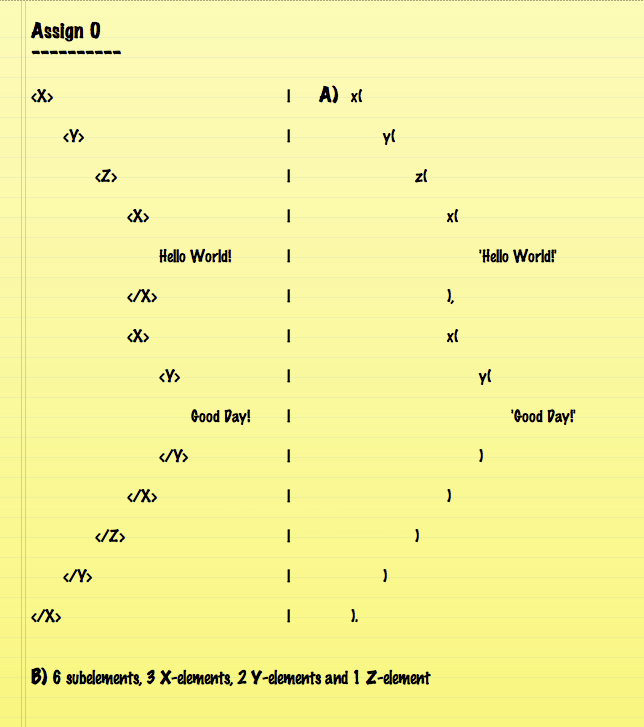
\includegraphics{assign0a.png}}
\caption{\emph{Left:} Construction of a non-trivial \emph{well-formed} XML instance using tag names
\code{x}, \code{y}, and \code{z}.  \emph{Right:} Prolog term \emph{pretty-printed} to align with the
XML tag elements on the left.  \emph{Bottom:} Answer to part \textbf{A} of assignment 0.}\end{figure}


\section{Part C}
\label{assign0:part-c}
\begin{notice}{note}{Todo}

Draw the node-labeled, (left-to-right-)ordered tree for which the XML element and equivalent Prolog structure are just two linearized representations. Hint: The vertical subelement/substructure extension corresponds to subtree breadth; the horizontal subelement/substructure indention corresponds to subtree depth.
\end{notice}

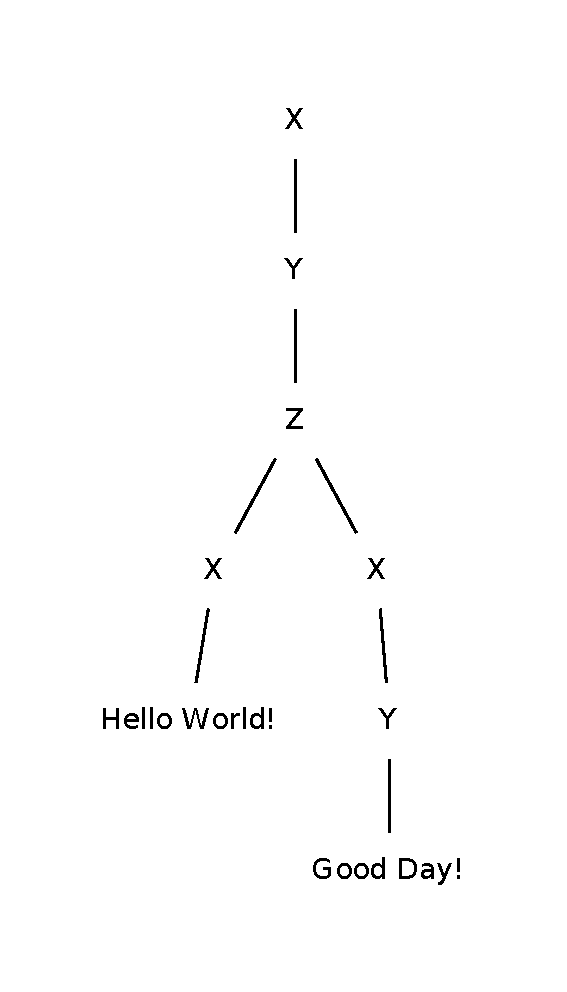
\includegraphics{graphviz-ca9411c629b22c9cf6cf6dc318a5b73a7efe365a.pdf}

Visualization of the XML isntance tree structure, \emph{rendered using Graphviz}.


\section{Part D}
\label{assign0:part-d}
\begin{notice}{note}{Todo}

List the notational (dis)advantages of the XML and Prolog representations.
\end{notice}

The notational advantages of xml representations are generally well known among programmers and are many (cf. {\hyperref[assign0:json]{{[}JSON{]}}}):
\begin{itemize}
\item {} 
XML is human readable.

\item {} 
XML can be used as an exchange/interchange format to enable users to mover thier data between similar applications.

\item {} 
XML provides structure to data so taht it is richer in information.

\item {} 
XML is easily processed because of the structure of the data is simple and standard.

\item {} 
There is a wide range of reusable software available to programmers to handle XML so they don't have to re-invent code.

\item {} 
XML seperates the presentation of data from the structure of that data.

\item {} 
Many views of the one data.

\item {} 
Self-describing data.

\item {} 
Complete integration of all traditional databases and formats.

\item {} 
Internationalization.

\item {} 
Open and extensible.

\item {} 
XML is widely adopted by the computer industry.

\end{itemize}

The notational disadvantages of xml representations are also generally well know to programmers (cf. {\hyperref[assign0:tolf11]{{[}Tolf11{]}}}):
\begin{itemize}
\item {} 
DOM is too specialized.

\item {} 
Can be cumbersome and inefficient.

\item {} 
Does not map well to data types of most programming languages.

\end{itemize}

The notational advantages of prolog representations are similar to those of XML in that they are human readable, they provide a structure to the data so that it is richer in information.

The notational disadvantages of prolog are inherent to all dynamically checked programming languages, e.g.: type checking done at run-time, only one datatype (\code{term}) (cf. {\hyperref[assign0:wp1]{{[}Wp1{]}}}).


\section{Part E}
\label{assign0:part-e}
\begin{notice}{note}{Todo}

Can anything be logically wrong with the legal Prolog structures corresponding to arbitrary XML elements that use repeated tags from \{x, y, z\}? Hint: Consider ways in which not only XML but also Prolog is ``less formal'' than logic (types, modes, arities, ...).
\end{notice}

XML and Prolog are less formal and their type specifications are much more relaxed than formal logics.  According to {\hyperref[assign0:brac04]{{[}Brac04{]}}} (chapter 2, p. 25) the aim of formal logics is to build up a \emph{Logical Model} such that the set of possible interpretations is made more narrow
so as to rule out more and more unintended interpretations.
Ultimately, logical consequene itself will tend toward ```truth in the intended interpretation'''.
The \emph{document object mode (DOM)} implemented by XML does not provide semantics for ``logical implications/inference/entailment'' the relationships between elements are structural only, and while a term can be expressed in \emph{Prolog} that mimics the structure of an
XML document queries against such terms are seem to be \emph{meaningless} and \emph{useless} since the inner terms are inaccessbile to the \code{top loop}.

\begin{tabular}{|p{0.950\linewidth}|}
\hline

Prolog REPL Sample
\\

\begin{OriginalVerbatim}[commandchars=\\\{\}]
?- \PYG{o}{[}\PYG{l+s+s1}{'Assign0.pl'}\PYG{o}{]}.
\PYGZpc{} Assign0.pl compiled 0.00 sec, 1,768 bytes
true.

?- listing.

a\PYG{o}{(}b\PYG{o}{(}c\PYG{o}{(}\PYG{l+s+s1}{'hello world'}\PYG{o}{)}\PYG{o}{)}\PYG{o}{)}.

x\PYG{o}{(}y\PYG{o}{(}z\PYG{o}{(}x\PYG{o}{(}\PYG{l+s+s1}{'hello world'}\PYG{o}{)}, x\PYG{o}{(}y\PYG{o}{(}hi\PYG{o}{)}\PYG{o}{)}\PYG{o}{)}\PYG{o}{)}\PYG{o}{)}.
true.

?- c\PYG{o}{(}X\PYG{o}{)}.
ERROR: toplevel: Undefined procedure: c/1 \PYG{o}{(}DWIM could not correct goal\PYG{o}{)}
?- z\PYG{o}{(}X\PYG{o}{)}.
ERROR: toplevel: Undefined procedure: z/1 \PYG{o}{(}DWIM could not correct goal\PYG{o}{)}
\end{OriginalVerbatim}
\\
\hline
\end{tabular}



\chapter{Lab 1 - Create your own XML DTD, XSD, and RNC or RNG}
\label{lab1:lab-1-create-your-own-xml-dtd-xsd-and-rnc-or-rng}\label{lab1::doc}
\begin{notice}{note}{Todo}

Consider these examples of XML documents for clause sets consisting of zero or
more facts f (Prolog: \code{f.}) and zero or more `backward' rules c \textless{}- p
(Prolog: \code{c :- p.}), in any order (``myurl'' will be replaced as explained below):

\begin{Verbatim}[commandchars=\\\{\}]
\PYG{c+cp}{\textless{}?xml version="1.0" standalone="no"?\textgreater{}}
\PYG{c+cp}{\textless{}!DOCTYPE clauses SYSTEM "myurl"\textgreater{}}
 \PYG{n+nt}{\textless{}clauses}\PYG{n+nt}{\textgreater{}}
    \PYG{n+nt}{\textless{}fact}\PYG{n+nt}{\textgreater{}} f \PYG{n+nt}{\textless{}/fact\textgreater{}}
    \PYG{n+nt}{\textless{}rule}\PYG{n+nt}{\textgreater{}} \PYG{n+nt}{\textless{}conc}\PYG{n+nt}{\textgreater{}} c \PYG{n+nt}{\textless{}/conc\textgreater{}} \PYG{n+nt}{\textless{}prem}\PYG{n+nt}{\textgreater{}} p \PYG{n+nt}{\textless{}/prem\textgreater{}} \PYG{n+nt}{\textless{}/rule\textgreater{}}
 \PYG{n+nt}{\textless{}/clauses\textgreater{}}

\PYG{c+cp}{\textless{}?xml version="1.0" standalone="no"?\textgreater{}}
\PYG{c+cp}{\textless{}!DOCTYPE clauses SYSTEM "myurl"\textgreater{}}
\PYG{n+nt}{\textless{}clauses}\PYG{n+nt}{\textgreater{}}
    \PYG{n+nt}{\textless{}rule}\PYG{n+nt}{\textgreater{}} \PYG{n+nt}{\textless{}conc}\PYG{n+nt}{\textgreater{}} c1 \PYG{n+nt}{\textless{}/conc\textgreater{}} \PYG{n+nt}{\textless{}prem}\PYG{n+nt}{\textgreater{}} p1 \PYG{n+nt}{\textless{}/prem\textgreater{}} \PYG{n+nt}{\textless{}/rule\textgreater{}}
    \PYG{n+nt}{\textless{}fact}\PYG{n+nt}{\textgreater{}} f1 \PYG{n+nt}{\textless{}/fact\textgreater{}}
    \PYG{n+nt}{\textless{}rule}\PYG{n+nt}{\textgreater{}} \PYG{n+nt}{\textless{}conc}\PYG{n+nt}{\textgreater{}} c2 \PYG{n+nt}{\textless{}/conc\textgreater{}} \PYG{n+nt}{\textless{}prem}\PYG{n+nt}{\textgreater{}} p2 \PYG{n+nt}{\textless{}/prem\textgreater{}} \PYG{n+nt}{\textless{}/rule\textgreater{}}
    \PYG{n+nt}{\textless{}fact}\PYG{n+nt}{\textgreater{}} f2 \PYG{n+nt}{\textless{}/fact\textgreater{}}
    \PYG{n+nt}{\textless{}fact}\PYG{n+nt}{\textgreater{}} f3 \PYG{n+nt}{\textless{}/fact\textgreater{}}
\PYG{n+nt}{\textless{}/clauses\textgreater{}}
\end{Verbatim}

Inductively complete this XML DTD (overwrite the ''...'' lines) for such clause sets:

\begin{Verbatim}[commandchars=\\\{\}]
\PYG{c+cp}{\textless{}!ELEMENT clauses   (................)\textgreater{}}
\PYG{c+cp}{\textless{}!ELEMENT rule   (................)\textgreater{}}
\PYG{c+cp}{\textless{}!ELEMENT fact    (\PYGZsh{}PCDATA)\textgreater{}}
\PYG{c+cp}{\textless{}!ELEMENT ........    (................)\textgreater{}}
\PYG{c+cp}{\textless{}!ELEMENT ........    (................)\textgreater{}}
\end{Verbatim}
\end{notice}


\section{DTD}
\label{lab1:dtd}
\begin{Verbatim}[commandchars=\\\{\}]
\PYG{c+cp}{\textless{}!ELEMENT clauses (fact\textbar{}rule)*\textgreater{}}
\PYG{c+cp}{\textless{}!ELEMENT rule                (conc,prem)\textgreater{}}
\PYG{c+cp}{\textless{}!ELEMENT fact                (\PYGZsh{}PCDATA)\textgreater{}}
\PYG{c+cp}{\textless{}!ELEMENT conc                (\PYGZsh{}PCDATA)\textgreater{}}
\PYG{c+cp}{\textless{}!ELEMENT prem                (\PYGZsh{}PCDATA)\textgreater{}}
\end{Verbatim}


\section{XSD}
\label{lab1:xsd}
\begin{Verbatim}[commandchars=\\\{\}]
\PYG{c+cp}{\textless{}?xml version="1.0"?\textgreater{}}
\PYG{n+nt}{\textless{}xs:schema} \PYG{n+na}{xmlns:xs=}\PYG{l+s}{"http://www.w3.org/2001/XMLSchema"}\PYG{n+nt}{\textgreater{}}
  \PYG{n+nt}{\textless{}xs:element} \PYG{n+na}{name=}\PYG{l+s}{"clauses"}\PYG{n+nt}{\textgreater{}}
    \PYG{n+nt}{\textless{}xs:complexType}\PYG{n+nt}{\textgreater{}}
      \PYG{n+nt}{\textless{}xs:sequence}\PYG{n+nt}{\textgreater{}}
        \PYG{n+nt}{\textless{}xs:choice} \PYG{n+na}{maxOccurs=}\PYG{l+s}{"unbounded"}\PYG{n+nt}{\textgreater{}}
          \PYG{n+nt}{\textless{}xs:element} \PYG{n+na}{ref=}\PYG{l+s}{"rule"}\PYG{n+nt}{/\textgreater{}}
          \PYG{n+nt}{\textless{}xs:element} \PYG{n+na}{ref=}\PYG{l+s}{"fact"}\PYG{n+nt}{/\textgreater{}}
        \PYG{n+nt}{\textless{}/xs:choice\textgreater{}}
      \PYG{n+nt}{\textless{}/xs:sequence\textgreater{}}
    \PYG{n+nt}{\textless{}/xs:complexType\textgreater{}}
  \PYG{n+nt}{\textless{}/xs:element\textgreater{}}
  \PYG{n+nt}{\textless{}xs:element} \PYG{n+na}{name=}\PYG{l+s}{"rule"}\PYG{n+nt}{\textgreater{}}
    \PYG{n+nt}{\textless{}xs:complexType}\PYG{n+nt}{\textgreater{}}
      \PYG{n+nt}{\textless{}xs:sequence}\PYG{n+nt}{\textgreater{}}
        \PYG{n+nt}{\textless{}xs:element} \PYG{n+na}{ref=}\PYG{l+s}{"conc"}\PYG{n+nt}{/\textgreater{}}
        \PYG{n+nt}{\textless{}xs:element} \PYG{n+na}{ref=}\PYG{l+s}{"prem"}\PYG{n+nt}{/\textgreater{}}
      \PYG{n+nt}{\textless{}/xs:sequence\textgreater{}}
    \PYG{n+nt}{\textless{}/xs:complexType\textgreater{}}
  \PYG{n+nt}{\textless{}/xs:element\textgreater{}}
  \PYG{n+nt}{\textless{}xs:element} \PYG{n+na}{name=}\PYG{l+s}{"fact"} \PYG{n+na}{type=}\PYG{l+s}{"xs:string"}\PYG{n+nt}{/\textgreater{}}
  \PYG{n+nt}{\textless{}xs:element} \PYG{n+na}{name=}\PYG{l+s}{"conc"} \PYG{n+na}{type=}\PYG{l+s}{"xs:string"}\PYG{n+nt}{/\textgreater{}}
  \PYG{n+nt}{\textless{}xs:element} \PYG{n+na}{name=}\PYG{l+s}{"prem"} \PYG{n+na}{type=}\PYG{l+s}{"xs:string"}\PYG{n+nt}{/\textgreater{}}
\PYG{n+nt}{\textless{}/xs:schema\textgreater{}}
\end{Verbatim}


\section{RelaxNG}
\label{lab1:relaxng}
Compact syntax:

\begin{Verbatim}[commandchars=@\[\]]
default namespace = ""

start = clauses
clauses = element clauses {
  (element rule {
    (element conc {xsd:string},
    element prem {xsd:string})}
  @textbar[] (element fact {xsd:string}))*}
\end{Verbatim}

\begin{notice}{note}{Note:}
I used \href{http://www.thaiopensource.com/relaxng/trang.html}{trang} to transform
RelaxNG compact syntax into xml-based syntax.
\end{notice}

XML syntax:

\begin{Verbatim}[commandchars=\\\{\}]
\PYG{c+cp}{\textless{}?xml version="1.0" encoding="UTF-8"?\textgreater{}}
\PYG{n+nt}{\textless{}grammar} \PYG{n+na}{ns=}\PYG{l+s}{""} \PYG{n+na}{xmlns=}\PYG{l+s}{"http://relaxng.org/ns/structure/1.0"} \PYG{n+na}{datatypeLibrary=}\PYG{l+s}{"http://www.w3.org/2001/XMLSchema-datatypes"}\PYG{n+nt}{\textgreater{}}
  \PYG{n+nt}{\textless{}start}\PYG{n+nt}{\textgreater{}}
    \PYG{n+nt}{\textless{}ref} \PYG{n+na}{name=}\PYG{l+s}{"clauses"}\PYG{n+nt}{/\textgreater{}}
  \PYG{n+nt}{\textless{}/start\textgreater{}}
  \PYG{n+nt}{\textless{}define} \PYG{n+na}{name=}\PYG{l+s}{"clauses"}\PYG{n+nt}{\textgreater{}}
    \PYG{n+nt}{\textless{}element} \PYG{n+na}{name=}\PYG{l+s}{"clauses"}\PYG{n+nt}{\textgreater{}}
      \PYG{n+nt}{\textless{}zeroOrMore}\PYG{n+nt}{\textgreater{}}
        \PYG{n+nt}{\textless{}choice}\PYG{n+nt}{\textgreater{}}
          \PYG{n+nt}{\textless{}element} \PYG{n+na}{name=}\PYG{l+s}{"rule"}\PYG{n+nt}{\textgreater{}}
            \PYG{n+nt}{\textless{}element} \PYG{n+na}{name=}\PYG{l+s}{"conc"}\PYG{n+nt}{\textgreater{}}
              \PYG{n+nt}{\textless{}data} \PYG{n+na}{type=}\PYG{l+s}{"string"}\PYG{n+nt}{/\textgreater{}}
            \PYG{n+nt}{\textless{}/element\textgreater{}}
            \PYG{n+nt}{\textless{}element} \PYG{n+na}{name=}\PYG{l+s}{"prem"}\PYG{n+nt}{\textgreater{}}
              \PYG{n+nt}{\textless{}data} \PYG{n+na}{type=}\PYG{l+s}{"string"}\PYG{n+nt}{/\textgreater{}}
            \PYG{n+nt}{\textless{}/element\textgreater{}}
          \PYG{n+nt}{\textless{}/element\textgreater{}}
          \PYG{n+nt}{\textless{}element} \PYG{n+na}{name=}\PYG{l+s}{"fact"}\PYG{n+nt}{\textgreater{}}
            \PYG{n+nt}{\textless{}data} \PYG{n+na}{type=}\PYG{l+s}{"string"}\PYG{n+nt}{/\textgreater{}}
          \PYG{n+nt}{\textless{}/element\textgreater{}}
        \PYG{n+nt}{\textless{}/choice\textgreater{}}
      \PYG{n+nt}{\textless{}/zeroOrMore\textgreater{}}
    \PYG{n+nt}{\textless{}/element\textgreater{}}
  \PYG{n+nt}{\textless{}/define\textgreater{}}
\PYG{n+nt}{\textless{}/grammar\textgreater{}}
\end{Verbatim}


\section{Misc}
\label{lab1:misc}
\begin{notice}{note}{Note:}
To validate the above sample instances I used \href{http://xmlsoft.org/xmllint.html}{xmllint - command line XML tool}
to parse and typecheck/validate:

\begin{Verbatim}[commandchars=\\\{\}]
\PYG{n+nv}{\PYGZdl{} }xmllint --noout --schema http://reubenpeterpaul.github.com/lab1/XSD/clauses.xsd clauses-instance.xml
\PYG{n+nv}{\PYGZdl{} }xmllint --noout --dtdvalid http://reubenpeterpaul.github.com/lab1/DTD/clauses.dtd clauses-instance.xml
\PYG{n+nv}{\PYGZdl{} }trang clauses.rnc clauses.rng
\PYG{n+nv}{\PYGZdl{} }xmllint --noout --relaxng http://reubenpeterpaul.github.com/lab1/DTD/clauses.rng clauses-instance.xml
\end{Verbatim}
\end{notice}

\begin{notice}{note}{Note:}
I also used my own custom \href{http://www.sagehill.net/docbookxsl/WriteCatalog.html}{XML catalog file}:

\begin{Verbatim}[commandchars=\\\{\}]
\PYG{c+cp}{\textless{}?xml version="1.0"?\textgreater{}}
\PYG{c+cp}{\textless{}!DOCTYPE catalog}
\PYG{c+cp}{PUBLIC "-//OASIS/DTD Entity Resolution XML Catalog V1.0//EN"}
\PYG{c+cp}{"http://www.oasis-open.org/committees/entity/release/1.0/catalog.dtd"\textgreater{}}
\PYG{n+nt}{\textless{}catalog}
\PYG{n+na}{xmlns=}\PYG{l+s}{"urn:oasis:names:tc:entity:xmlns:xml:catalog"}\PYG{n+nt}{\textgreater{}}

...

  \PYG{n+nt}{\textless{}system}
  \PYG{n+na}{systemId=}\PYG{l+s}{"http://reubenpeterpaul.github.com/cs6795/lab1/DTD/clauses.dtd"}
  \PYG{n+na}{uri=}\PYG{l+s}{"/home/peter-paulr/.laboratory/cs6795/lab1/clauses.dtd"}
  \PYG{n+nt}{/\textgreater{}}

  \PYG{n+nt}{\textless{}system}
  \PYG{n+na}{systemId=}\PYG{l+s}{"http://reubenpeterpaul.github.com/cs6795/lab1/XSD/clauses.xsd"}
  \PYG{n+na}{uri=}\PYG{l+s}{"/home/peter-paulr/.laboratory/cs6795/lab1/clauses.xsd"}
  \PYG{n+nt}{/\textgreater{}}

  \PYG{n+nt}{\textless{}system}
  \PYG{n+na}{systemId=}\PYG{l+s}{"http://reubenpeterpaul.github.com/cs6795/lab1/RNG/clauses.rng"}
  \PYG{n+na}{uri=}\PYG{l+s}{"/home/peter-paulr/.laboratory/cs6795/lab1/clauses.rng"}
  \PYG{n+nt}{/\textgreater{}}
\PYG{n+nt}{\textless{}/catalog\textgreater{}}
\end{Verbatim}
\end{notice}


\chapter{Assignment 1}
\label{assign1:assignment-1}\label{assign1::doc}
\begin{notice}{note}{Note:}
Please mark after parts {\hyperref[assign1:a1]{\emph{Part A-1}}} and {\hyperref[assign1:a2]{\emph{Part A-2}}}.
\end{notice}


\section{Part A-0}
\label{assign1:part-a-0}
\begin{notice}{note}{Todo}

Do the missing leaf data for passengers cause any
(XML-level) issue?
\end{notice}

No the the missing leaf data (\code{\#PCDATA}) does not affect the xml
well-formedness.


\section{Part A-1}
\label{assign1:a1}\label{assign1:part-a-1}
\begin{notice}{note}{Todo}

Does the repeatedly occurring \code{appellation}:

\begin{Verbatim}[commandchars=\\\{\}]
\PYG{n+nf}{appellation}\PYG{p}{(}\PYG{l+s+sAtom}{'Main St'}\PYG{p}{)}\PYG{p}{.}     \PYG{n+nf}{appellation}\PYG{p}{(}\PYG{l+s+sAtom}{'Fredericton'}\PYG{p}{)}\PYG{p}{.}
\end{Verbatim}

label cause a problem with respect to the unambiguous representation of
all parts of the taxi-ride information?
Hint: Is it even necessary to check whether every leaf of the tree -
ordered  from 37 to 12.50 - are uniquely denoted by the ``path name'' of node
labels leading to it from the taxi-ride root? What about any other repeatedly
occurring label?
\end{notice}

To determine potential ambiguity introduced by the repeated use of the
\code{appellation} tag-label consider the following prolog system:

\begin{Verbatim}[commandchars=\\\{\}]
\PYG{n+nf}{appellation}\PYG{p}{(}\PYG{l+s+sAtom}{'Main St'}\PYG{p}{)}\PYG{p}{.}
\PYG{n+nf}{appellation}\PYG{p}{(}\PYG{l+s+sAtom}{'Fredericton'}\PYG{p}{)}\PYG{p}{.}
\PYG{n+nf}{first}\PYG{p}{(}\PYG{l+s+sAtom}{'Peter'}\PYG{p}{)}\PYG{p}{.}
\PYG{n+nf}{mid}\PYG{p}{(}\PYG{l+s+sAtom}{'C.'}\PYG{p}{)}\PYG{p}{.}
\PYG{n+nf}{lastn}\PYG{p}{(}\PYG{l+s+sAtom}{'Jones'}\PYG{p}{)}\PYG{p}{.}
\PYG{n+nf}{numbern}\PYG{p}{(}\PYG{l+m}{37}\PYG{p}{)}\PYG{p}{.}
\PYG{n+nf}{numbern}\PYG{p}{(}\PYG{l+m}{12}\PYG{p}{)}\PYG{p}{.}
\PYG{n+nf}{province}\PYG{p}{(}\PYG{l+s+sAtom}{'NB'}\PYG{p}{)}\PYG{p}{.}

\PYG{n+nf}{name}\PYG{p}{(}\PYG{n+nv}{X}\PYG{p}{,}\PYG{n+nv}{Y}\PYG{p}{,}\PYG{n+nv}{Z}\PYG{p}{)} \PYG{p}{:-} \PYG{n+nf}{first}\PYG{p}{(}\PYG{n+nv}{X}\PYG{p}{)}\PYG{p}{,} \PYG{n+nf}{mid}\PYG{p}{(}\PYG{n+nv}{Y}\PYG{p}{)}\PYG{p}{,} \PYG{n+nf}{lastn}\PYG{p}{(}\PYG{n+nv}{Z}\PYG{p}{)}\PYG{p}{.}
\PYG{n+nf}{driver}\PYG{p}{(}\PYG{n+nv}{W}\PYG{p}{,}\PYG{n+nv}{X}\PYG{p}{,}\PYG{n+nv}{Y}\PYG{p}{,}\PYG{n+nv}{Z}\PYG{p}{)} \PYG{p}{:-} \PYG{n+nf}{numbern}\PYG{p}{(}\PYG{n+nv}{W}\PYG{p}{)}\PYG{p}{,} \PYG{n+nf}{name}\PYG{p}{(}\PYG{n+nv}{X}\PYG{p}{,}\PYG{n+nv}{Y}\PYG{p}{,}\PYG{n+nv}{Z}\PYG{p}{)}\PYG{p}{.}
\PYG{n+nf}{municipality}\PYG{p}{(}\PYG{n+nv}{X}\PYG{p}{,}\PYG{n+nv}{Y}\PYG{p}{)} \PYG{p}{:-} \PYG{n+nf}{appellation}\PYG{p}{(}\PYG{n+nv}{X}\PYG{p}{)}\PYG{p}{,} \PYG{n+nf}{province}\PYG{p}{(}\PYG{n+nv}{Y}\PYG{p}{)}\PYG{p}{.}
\PYG{n+nf}{street}\PYG{p}{(}\PYG{n+nv}{X}\PYG{p}{,}\PYG{n+nv}{Y}\PYG{p}{)} \PYG{p}{:-} \PYG{n+nf}{number}\PYG{p}{(}\PYG{n+nv}{X}\PYG{p}{)}\PYG{p}{,} \PYG{n+nf}{appellation}\PYG{p}{(}\PYG{n+nv}{Y}\PYG{p}{)}\PYG{p}{.}
\end{Verbatim}

Backtracking in prolog against the query \code{street(X,Y)} yields the
following results:

\begin{Verbatim}[commandchars=\\\{\}]
?- \PYG{o}{[}\PYG{l+s+s1}{'testA2'}\PYG{o}{]}.
\PYGZpc{} testA2 compiled 0.00 sec, 5,624 bytes
true.

?- street\PYG{o}{(}X,Y\PYG{o}{)}.
\PYG{n+nv}{X} \PYG{o}{=} 37,
\PYG{n+nv}{Y} \PYG{o}{=} \PYG{l+s+s1}{'Main St'} ;
\PYG{n+nv}{X} \PYG{o}{=} 37,
\PYG{n+nv}{Y} \PYG{o}{=} \PYG{l+s+s1}{'Fredericton'} ;
\PYG{n+nv}{X} \PYG{o}{=} 12,
\PYG{n+nv}{Y} \PYG{o}{=} \PYG{l+s+s1}{'Main St'} ;
\PYG{n+nv}{X} \PYG{o}{=} 12,
\PYG{n+nv}{Y} \PYG{o}{=} \PYG{l+s+s1}{'Fredericton'}.
\end{Verbatim}

This illustrates by example that the repeated use of \code{appellation} and also
\code{number} results in adding ambiguity to the representation of \code{taxi-ride}.
This problem can be dealt with via introduction of complex types, or denoting
the leaf nodes with the path of node-labels from the root \code{taxi-ride}, e.g.:

\begin{Verbatim}[commandchars=\\\{\}]
\PYG{n+nf}{street}\PYG{p}{(}\PYG{n+nf}{numbern}\PYG{p}{(}\PYG{l+m}{12}\PYG{p}{)}\PYG{p}{,} \PYG{n+nf}{appellation}\PYG{p}{(}\PYG{l+s+sAtom}{'Main St'}\PYG{p}{)}\PYG{p}{)}\PYG{p}{.}
\PYG{n+nf}{municipality}\PYG{p}{(}\PYG{n+nf}{appellation}\PYG{p}{(}\PYG{l+s+sAtom}{'Fredericton'}\PYG{p}{)}\PYG{p}{,} \PYG{n+nf}{province}\PYG{p}{(}\PYG{l+s+sAtom}{'NB'}\PYG{p}{)}\PYG{p}{)}\PYG{p}{.}
\end{Verbatim}


\section{Part A-2}
\label{assign1:part-a-2}\label{assign1:a2}
\begin{notice}{note}{Todo}

What if the nodes labeled `appellation' would have been labeled `name',
too?
\end{notice}

Again let us consider a prolog system:

\begin{Verbatim}[commandchars=\\\{\}]
\PYG{n+nf}{name}\PYG{p}{(}\PYG{l+s+sAtom}{'Main St'}\PYG{p}{)}\PYG{p}{.}
\PYG{n+nf}{name}\PYG{p}{(}\PYG{l+s+sAtom}{'Fredericton'}\PYG{p}{)}\PYG{p}{.}
\PYG{n+nf}{first}\PYG{p}{(}\PYG{l+s+sAtom}{'Peter'}\PYG{p}{)}\PYG{p}{.}
\PYG{n+nf}{mid}\PYG{p}{(}\PYG{l+s+sAtom}{'C.'}\PYG{p}{)}\PYG{p}{.}
\PYG{n+nf}{lastn}\PYG{p}{(}\PYG{l+s+sAtom}{'Jones'}\PYG{p}{)}\PYG{p}{.}
\PYG{n+nf}{numbern}\PYG{p}{(}\PYG{l+m}{37}\PYG{p}{)}\PYG{p}{.}
\PYG{n+nf}{numbern}\PYG{p}{(}\PYG{l+m}{12}\PYG{p}{)}\PYG{p}{.}
\PYG{n+nf}{province}\PYG{p}{(}\PYG{l+s+sAtom}{'NB'}\PYG{p}{)}\PYG{p}{.}

\PYG{n+nf}{name}\PYG{p}{(}\PYG{n+nv}{X}\PYG{p}{,}\PYG{n+nv}{Y}\PYG{p}{,}\PYG{n+nv}{Z}\PYG{p}{)} \PYG{p}{:-} \PYG{n+nf}{first}\PYG{p}{(}\PYG{n+nv}{X}\PYG{p}{)}\PYG{p}{,} \PYG{n+nf}{mid}\PYG{p}{(}\PYG{n+nv}{Y}\PYG{p}{)}\PYG{p}{,} \PYG{n+nf}{lastn}\PYG{p}{(}\PYG{n+nv}{Z}\PYG{p}{)}\PYG{p}{.}
\PYG{n+nf}{driver}\PYG{p}{(}\PYG{n+nv}{W}\PYG{p}{,}\PYG{n+nv}{X}\PYG{p}{,}\PYG{n+nv}{Y}\PYG{p}{,}\PYG{n+nv}{Z}\PYG{p}{)} \PYG{p}{:-} \PYG{n+nf}{numbern}\PYG{p}{(}\PYG{n+nv}{W}\PYG{p}{)}\PYG{p}{,} \PYG{n+nf}{name}\PYG{p}{(}\PYG{n+nv}{X}\PYG{p}{,}\PYG{n+nv}{Y}\PYG{p}{,}\PYG{n+nv}{Z}\PYG{p}{)}\PYG{p}{.}
\PYG{n+nf}{municipality}\PYG{p}{(}\PYG{n+nv}{X}\PYG{p}{,}\PYG{n+nv}{Y}\PYG{p}{)} \PYG{p}{:-} \PYG{n+nf}{name}\PYG{p}{(}\PYG{n+nv}{X}\PYG{p}{)}\PYG{p}{,} \PYG{n+nf}{province}\PYG{p}{(}\PYG{n+nv}{Y}\PYG{p}{)}\PYG{p}{.}
\PYG{n+nf}{street}\PYG{p}{(}\PYG{n+nv}{X}\PYG{p}{,}\PYG{n+nv}{Y}\PYG{p}{)} \PYG{p}{:-} \PYG{n+nf}{number}\PYG{p}{(}\PYG{n+nv}{X}\PYG{p}{)}\PYG{p}{,} \PYG{n+nf}{name}\PYG{p}{(}\PYG{n+nv}{Y}\PYG{p}{)}\PYG{p}{.}
\end{Verbatim}

Backtracaking in prolog REPL against the query \code{street} and \code{driver}
yields the following results:

\begin{Verbatim}[commandchars=\\\{\}]
\PYG{l+s+sAtom}{?-} \PYG{n+nf}{consult}\PYG{p}{(}\PYG{l+s+sAtom}{'testA2b'}\PYG{p}{)}\PYG{p}{.}
\PYG{c+c1}{\PYGZpc{} testA2b compiled 0.00 sec, 5,096 bytes}
\PYG{l+s+sAtom}{true}\PYG{p}{.}


\PYG{l+s+sAtom}{?-} \PYG{n+nf}{street}\PYG{p}{(}\PYG{n+nv}{X}\PYG{p}{,}\PYG{n+nv}{Y}\PYG{p}{)}\PYG{p}{.}
\PYG{n+nv}{X} \PYG{o}{=} \PYG{l+m}{37}\PYG{p}{,}
\PYG{n+nv}{Y} \PYG{o}{=} \PYG{l+s+sAtom}{'Main St'} \PYG{p}{;}
\PYG{n+nv}{X} \PYG{o}{=} \PYG{l+m}{37}\PYG{p}{,}
\PYG{n+nv}{Y} \PYG{o}{=} \PYG{l+s+sAtom}{'Fredericton'} \PYG{p}{;}
\PYG{n+nv}{X} \PYG{o}{=} \PYG{l+m}{12}\PYG{p}{,}
\PYG{n+nv}{Y} \PYG{o}{=} \PYG{l+s+sAtom}{'Main St'} \PYG{p}{;}
\PYG{n+nv}{X} \PYG{o}{=} \PYG{l+m}{12}\PYG{p}{,}
\PYG{n+nv}{Y} \PYG{o}{=} \PYG{l+s+sAtom}{'Fredericton'}\PYG{p}{.}

\PYG{l+s+sAtom}{?-} \PYG{n+nf}{driver}\PYG{p}{(}\PYG{n+nv}{W}\PYG{p}{,}\PYG{n+nv}{X}\PYG{p}{,}\PYG{n+nv}{Y}\PYG{p}{,}\PYG{n+nv}{Z}\PYG{p}{)}\PYG{p}{.}
\PYG{n+nv}{W} \PYG{o}{=} \PYG{l+m}{37}\PYG{p}{,}
\PYG{n+nv}{X} \PYG{o}{=} \PYG{l+s+sAtom}{'Peter'}\PYG{p}{,}
\PYG{n+nv}{Y} \PYG{o}{=} \PYG{l+s+sAtom}{'C.'}\PYG{p}{,}
\PYG{n+nv}{Z} \PYG{o}{=} \PYG{l+s+sAtom}{'Jones'}\PYG{p}{.}
\PYG{n+nv}{W} \PYG{o}{=} \PYG{l+m}{12}\PYG{p}{,}
\PYG{n+nv}{X} \PYG{o}{=} \PYG{l+s+sAtom}{'Peter'}\PYG{p}{,}
\PYG{n+nv}{Y} \PYG{o}{=} \PYG{l+s+sAtom}{'C.'}\PYG{p}{,}
\PYG{n+nv}{Z} \PYG{o}{=} \PYG{l+s+sAtom}{'Jones'}\PYG{p}{.}
\end{Verbatim}

The result is the same as above ({\hyperref[assign1:a1]{\emph{Part A-1}}}).  \code{Node-labelled} paths are still
required to denotate the \code{name} tags used by \code{street} and \code{municipality}
nodes.  While the rule for \code{name} satisfies the complex conditions for
separating the parts of an individuals name.


\section{Part A-3 - Relabeling of tree in Prolog}
\label{assign1:part-a-3-relabeling-of-tree-in-prolog}
\begin{Verbatim}[commandchars=\\\{\}]
\PYG{n+nf}{carnumber}\PYG{p}{(}\PYG{l+m}{37}\PYG{p}{)}\PYG{p}{.}
\PYG{n+nf}{firstname}\PYG{p}{(}\PYG{l+s+sAtom}{'Peter'}\PYG{p}{)}\PYG{p}{.}
\PYG{n+nf}{middlename}\PYG{p}{(}\PYG{l+s+sAtom}{'C.'}\PYG{p}{)}\PYG{p}{.}
\PYG{n+nf}{lastname}\PYG{p}{(}\PYG{l+s+sAtom}{'Jones'}\PYG{p}{)}\PYG{p}{.}
\PYG{n+nf}{date}\PYG{p}{(}\PYG{l+s+sAtom}{'9/27'}\PYG{p}{)}\PYG{p}{.}
\PYG{n+nf}{streetnumber}\PYG{p}{(}\PYG{l+m}{12}\PYG{p}{)}\PYG{p}{.}
\PYG{n+nf}{streetname}\PYG{p}{(}\PYG{l+s+sAtom}{'Main St'}\PYG{p}{)}\PYG{p}{.}
\PYG{n+nf}{municipalityname}\PYG{p}{(}\PYG{l+s+sAtom}{'Fredericton'}\PYG{p}{)}\PYG{p}{.}
\PYG{n+nf}{provincename}\PYG{p}{(}\PYG{l+s+sAtom}{'NB'}\PYG{p}{)}\PYG{p}{.}
\PYG{n+nf}{fare}\PYG{p}{(}\PYG{l+m}{12}\PYG{p}{.}\PYG{l+m}{50}\PYG{p}{)}\PYG{p}{.}

\PYG{n+nf}{taxiride}\PYG{p}{(}\PYG{n+nv}{W}\PYG{p}{,}\PYG{n+nv}{X}\PYG{p}{,}\PYG{n+nv}{Y}\PYG{p}{,}\PYG{n+nv}{Z}\PYG{p}{,}\PYG{n+nv}{D}\PYG{p}{,}\PYG{n+nv}{E}\PYG{p}{,}\PYG{n+nv}{F}\PYG{p}{,}\PYG{n+nv}{G}\PYG{p}{,}\PYG{n+nv}{H}\PYG{p}{,}\PYG{n+nv}{I}\PYG{p}{)} \PYG{p}{:-}
  \PYG{n+nf}{driver}\PYG{p}{(}\PYG{n+nv}{W}\PYG{p}{,}\PYG{n+nv}{X}\PYG{p}{,}\PYG{n+nv}{Y}\PYG{p}{,}\PYG{n+nv}{Z}\PYG{p}{)}\PYG{p}{,}
  \PYG{l+s+sAtom}{passengers}\PYG{p}{,}
  \PYG{n+nf}{transportinformation}\PYG{p}{(}\PYG{n+nv}{D}\PYG{p}{,}\PYG{n+nv}{E}\PYG{p}{,}\PYG{n+nv}{F}\PYG{p}{,}\PYG{n+nv}{G}\PYG{p}{,}\PYG{n+nv}{H}\PYG{p}{,}\PYG{n+nv}{I}\PYG{p}{)}\PYG{p}{.}

\PYG{n+nf}{driver}\PYG{p}{(}\PYG{n+nv}{W}\PYG{p}{,}\PYG{n+nv}{X}\PYG{p}{,}\PYG{n+nv}{Y}\PYG{p}{,}\PYG{n+nv}{Z}\PYG{p}{)} \PYG{p}{:-} \PYG{n+nf}{carnumber}\PYG{p}{(}\PYG{n+nv}{W}\PYG{p}{)}\PYG{p}{,} \PYG{n+nf}{fullname}\PYG{p}{(}\PYG{n+nv}{X}\PYG{p}{,}\PYG{n+nv}{Y}\PYG{p}{,}\PYG{n+nv}{Z}\PYG{p}{)}\PYG{p}{.}

\PYG{n+nf}{fullname}\PYG{p}{(}\PYG{n+nv}{X}\PYG{p}{,}\PYG{n+nv}{Y}\PYG{p}{,}\PYG{n+nv}{Z}\PYG{p}{)} \PYG{p}{:-} \PYG{n+nf}{firstname}\PYG{p}{(}\PYG{n+nv}{X}\PYG{p}{)}\PYG{p}{,} \PYG{n+nf}{middlename}\PYG{p}{(}\PYG{n+nv}{Y}\PYG{p}{)}\PYG{p}{,} \PYG{n+nf}{lastname}\PYG{p}{(}\PYG{n+nv}{Z}\PYG{p}{)}\PYG{p}{.}

\PYG{n+nf}{transportinformation}\PYG{p}{(}\PYG{n+nv}{D}\PYG{p}{,}\PYG{n+nv}{E}\PYG{p}{,}\PYG{n+nv}{F}\PYG{p}{,}\PYG{n+nv}{G}\PYG{p}{,}\PYG{n+nv}{H}\PYG{p}{,}\PYG{n+nv}{I}\PYG{p}{)} \PYG{p}{:-} \PYG{n+nf}{date}\PYG{p}{(}\PYG{n+nv}{D}\PYG{p}{)}\PYG{p}{,} \PYG{n+nf}{destination}\PYG{p}{(}\PYG{n+nv}{E}\PYG{p}{,}\PYG{n+nv}{F}\PYG{p}{,}\PYG{n+nv}{G}\PYG{p}{,}\PYG{n+nv}{H}\PYG{p}{)}\PYG{p}{,}
\PYG{n+nf}{fare}\PYG{p}{(}\PYG{n+nv}{I}\PYG{p}{)}\PYG{p}{.}

\PYG{n+nf}{destination}\PYG{p}{(}\PYG{n+nv}{E}\PYG{p}{,}\PYG{n+nv}{F}\PYG{p}{,}\PYG{n+nv}{G}\PYG{p}{,}\PYG{n+nv}{H}\PYG{p}{)} \PYG{p}{:-} \PYG{n+nf}{street}\PYG{p}{(}\PYG{n+nv}{E}\PYG{p}{,}\PYG{n+nv}{F}\PYG{p}{)}\PYG{p}{,} \PYG{n+nf}{municipality}\PYG{p}{(}\PYG{n+nv}{G}\PYG{p}{,}\PYG{n+nv}{H}\PYG{p}{)}\PYG{p}{.}

\PYG{n+nf}{street}\PYG{p}{(}\PYG{n+nv}{X}\PYG{p}{,}\PYG{n+nv}{Y}\PYG{p}{)} \PYG{p}{:-} \PYG{n+nf}{streetnumber}\PYG{p}{(}\PYG{n+nv}{X}\PYG{p}{)}\PYG{p}{,} \PYG{n+nf}{streetname}\PYG{p}{(}\PYG{n+nv}{Y}\PYG{p}{)}\PYG{p}{.}

\PYG{n+nf}{municipality}\PYG{p}{(}\PYG{n+nv}{X}\PYG{p}{,}\PYG{n+nv}{Y}\PYG{p}{)} \PYG{p}{:-} \PYG{n+nf}{municipalityname}\PYG{p}{(}\PYG{n+nv}{X}\PYG{p}{)}\PYG{p}{,} \PYG{n+nf}{provincename}\PYG{p}{(}\PYG{n+nv}{Y}\PYG{p}{)}\PYG{p}{.}
\end{Verbatim}


\section{Part B-1 - Well formed XML element from \emph{Part A-1}}
\label{assign1:part-b-1-well-formed-xml-element-from-a1}
\begin{Verbatim}[commandchars=\\\{\}]
\PYG{c+cp}{\textless{}?xml version="1.0" ?\textgreater{}}
\PYG{n+nt}{\textless{}taxi-ride}\PYG{n+nt}{\textgreater{}}
  \PYG{n+nt}{\textless{}driver}\PYG{n+nt}{\textgreater{}}
    \PYG{n+nt}{\textless{}number}\PYG{n+nt}{\textgreater{}}37\PYG{n+nt}{\textless{}/number\textgreater{}}
    \PYG{n+nt}{\textless{}name}\PYG{n+nt}{\textgreater{}}
      \PYG{n+nt}{\textless{}first}\PYG{n+nt}{\textgreater{}}Peter\PYG{n+nt}{\textless{}/first\textgreater{}}
      \PYG{n+nt}{\textless{}mid}\PYG{n+nt}{\textgreater{}}C.\PYG{n+nt}{\textless{}/mid\textgreater{}}
      \PYG{n+nt}{\textless{}last}\PYG{n+nt}{\textgreater{}}Jones\PYG{n+nt}{\textless{}/last\textgreater{}}
    \PYG{n+nt}{\textless{}/name\textgreater{}}
  \PYG{n+nt}{\textless{}/driver\textgreater{}}
  \PYG{n+nt}{\textless{}passengers} \PYG{n+nt}{/\textgreater{}}
  \PYG{n+nt}{\textless{}tranport-information}\PYG{n+nt}{\textgreater{}}
    \PYG{n+nt}{\textless{}date}\PYG{n+nt}{\textgreater{}}9/27\PYG{n+nt}{\textless{}/date\textgreater{}}
    \PYG{n+nt}{\textless{}street}\PYG{n+nt}{\textgreater{}}
      \PYG{n+nt}{\textless{}number}\PYG{n+nt}{\textgreater{}}12\PYG{n+nt}{\textless{}/number\textgreater{}}
      \PYG{n+nt}{\textless{}appellation}\PYG{n+nt}{\textgreater{}}Main St\PYG{n+nt}{\textless{}/appellation\textgreater{}}
    \PYG{n+nt}{\textless{}/street\textgreater{}}
    \PYG{n+nt}{\textless{}municipality}\PYG{n+nt}{\textgreater{}}
      \PYG{n+nt}{\textless{}appellation}\PYG{n+nt}{\textgreater{}}Fredericton\PYG{n+nt}{\textless{}/appellation\textgreater{}}
      \PYG{n+nt}{\textless{}province}\PYG{n+nt}{\textgreater{}}NB\PYG{n+nt}{\textless{}/province\textgreater{}}
    \PYG{n+nt}{\textless{}/municipality\textgreater{}}
    \PYG{n+nt}{\textless{}fare}\PYG{n+nt}{\textgreater{}}
      12.50
    \PYG{n+nt}{\textless{}/fare\textgreater{}}
  \PYG{n+nt}{\textless{}/tranport-information\textgreater{}}
\PYG{n+nt}{\textless{}/taxi-ride\textgreater{}}
\end{Verbatim}

\emph{Yes}, a well formed XML instance can be given for {\hyperref[assign1:a1]{\emph{Part A-1}}}


\section{Part B-2 - Well formed XML element from \emph{Part A-2}}
\label{assign1:part-b-2-well-formed-xml-element-from-a2}
\begin{Verbatim}[commandchars=\\\{\}]
\PYG{c+cp}{\textless{}?xml version="1.0" ?\textgreater{}}
\PYG{n+nt}{\textless{}taxi-ride}\PYG{n+nt}{\textgreater{}}
  \PYG{n+nt}{\textless{}driver}\PYG{n+nt}{\textgreater{}}
    \PYG{n+nt}{\textless{}number}\PYG{n+nt}{\textgreater{}}37\PYG{n+nt}{\textless{}/number\textgreater{}}
    \PYG{n+nt}{\textless{}name}\PYG{n+nt}{\textgreater{}}
      \PYG{n+nt}{\textless{}first}\PYG{n+nt}{\textgreater{}}Peter\PYG{n+nt}{\textless{}/first\textgreater{}}
      \PYG{n+nt}{\textless{}mid}\PYG{n+nt}{\textgreater{}}C.\PYG{n+nt}{\textless{}/mid\textgreater{}}
      \PYG{n+nt}{\textless{}last}\PYG{n+nt}{\textgreater{}}Jones\PYG{n+nt}{\textless{}/last\textgreater{}}
    \PYG{n+nt}{\textless{}/name\textgreater{}}
  \PYG{n+nt}{\textless{}/driver\textgreater{}}
  \PYG{n+nt}{\textless{}passengers} \PYG{n+nt}{/\textgreater{}}
  \PYG{n+nt}{\textless{}tranport-information}\PYG{n+nt}{\textgreater{}}
    \PYG{n+nt}{\textless{}date}\PYG{n+nt}{\textgreater{}}9/27\PYG{n+nt}{\textless{}/date\textgreater{}}
    \PYG{n+nt}{\textless{}street}\PYG{n+nt}{\textgreater{}}
      \PYG{n+nt}{\textless{}number}\PYG{n+nt}{\textgreater{}}12\PYG{n+nt}{\textless{}/number\textgreater{}}
      \PYG{n+nt}{\textless{}name}\PYG{n+nt}{\textgreater{}}Main St\PYG{n+nt}{\textless{}/name\textgreater{}}
    \PYG{n+nt}{\textless{}/street\textgreater{}}
    \PYG{n+nt}{\textless{}municipality}\PYG{n+nt}{\textgreater{}}
      \PYG{n+nt}{\textless{}name}\PYG{n+nt}{\textgreater{}}Fredericton\PYG{n+nt}{\textless{}/name\textgreater{}}
      \PYG{n+nt}{\textless{}province}\PYG{n+nt}{\textgreater{}}NB\PYG{n+nt}{\textless{}/province\textgreater{}}
    \PYG{n+nt}{\textless{}/municipality\textgreater{}}
    \PYG{n+nt}{\textless{}fare}\PYG{n+nt}{\textgreater{}}
      12.50
    \PYG{n+nt}{\textless{}/fare\textgreater{}}
  \PYG{n+nt}{\textless{}/tranport-information\textgreater{}}
\PYG{n+nt}{\textless{}/taxi-ride\textgreater{}}
\end{Verbatim}

\emph{Yes}, a well formed XML instance can be given for {\hyperref[assign1:a2]{\emph{Part A-2}}}


\section{Part B-3 - XML instance of relabeling}
\label{assign1:part-b-3-xml-instance-of-relabeling}\label{assign1:b3}
\begin{Verbatim}[commandchars=\\\{\}]
\PYG{n+nt}{\textless{}taxiride}\PYG{n+nt}{\textgreater{}}
  \PYG{n+nt}{\textless{}driver}\PYG{n+nt}{\textgreater{}}
    \PYG{n+nt}{\textless{}carnumber}\PYG{n+nt}{\textgreater{}}37\PYG{n+nt}{\textless{}/carnumber\textgreater{}}
    \PYG{n+nt}{\textless{}fullname}\PYG{n+nt}{\textgreater{}}
      \PYG{n+nt}{\textless{}firstname}\PYG{n+nt}{\textgreater{}}Peter\PYG{n+nt}{\textless{}/firstname\textgreater{}}
      \PYG{n+nt}{\textless{}middlename}\PYG{n+nt}{\textgreater{}}C.\PYG{n+nt}{\textless{}/middlename\textgreater{}}
      \PYG{n+nt}{\textless{}lastname}\PYG{n+nt}{\textgreater{}}Jones\PYG{n+nt}{\textless{}/lastname\textgreater{}}
    \PYG{n+nt}{\textless{}/fullname\textgreater{}}
  \PYG{n+nt}{\textless{}/driver\textgreater{}}
  \PYG{n+nt}{\textless{}passengers} \PYG{n+nt}{/\textgreater{}}
  \PYG{n+nt}{\textless{}transportinformation}\PYG{n+nt}{\textgreater{}}
    \PYG{n+nt}{\textless{}date}\PYG{n+nt}{\textgreater{}}9/27\PYG{n+nt}{\textless{}/date\textgreater{}}
    \PYG{n+nt}{\textless{}detination}\PYG{n+nt}{\textgreater{}}
      \PYG{n+nt}{\textless{}street}\PYG{n+nt}{\textgreater{}}
        \PYG{n+nt}{\textless{}streetnumber}\PYG{n+nt}{\textgreater{}}12\PYG{n+nt}{\textless{}/streetnumber\textgreater{}}
        \PYG{n+nt}{\textless{}streetname}\PYG{n+nt}{\textgreater{}}Main St\PYG{n+nt}{\textless{}/streetname\textgreater{}}
      \PYG{n+nt}{\textless{}/street\textgreater{}}
      \PYG{n+nt}{\textless{}municipality}\PYG{n+nt}{\textgreater{}}
        \PYG{n+nt}{\textless{}municipalityname}\PYG{n+nt}{\textgreater{}}Fredericton\PYG{n+nt}{\textless{}/municipalityname\textgreater{}}
        \PYG{n+nt}{\textless{}provincename}\PYG{n+nt}{\textgreater{}}NB\PYG{n+nt}{\textless{}/provincename\textgreater{}}
      \PYG{n+nt}{\textless{}/municipality\textgreater{}}
    \PYG{n+nt}{\textless{}/destination\textgreater{}}
    \PYG{n+nt}{\textless{}fare}\PYG{n+nt}{\textgreater{}}12.50\PYG{n+nt}{\textless{}/fare\textgreater{}}
  \PYG{n+nt}{\textless{}/transportinformation\textgreater{}}
\PYG{n+nt}{\textless{}/taxiride\textgreater{}}
\end{Verbatim}


\section{Part C - Prolog equivalent term of \emph{Part B-3 - XML instance of relabeling}}
\label{assign1:part-c-prolog-equivalent-term-of-b3}
\begin{Verbatim}[commandchars=\\\{\}]
\PYG{n+nf}{taxiride}\PYG{p}{(}
  \PYG{n+nf}{driver}\PYG{p}{(}
    \PYG{n+nf}{carnumber}\PYG{p}{(}\PYG{l+m}{37}\PYG{p}{)}\PYG{p}{,}
    \PYG{n+nf}{fullname}\PYG{p}{(}
      \PYG{n+nf}{firstname}\PYG{p}{(}\PYG{l+s+sAtom}{'Peter'}\PYG{p}{)}\PYG{p}{,}
      \PYG{n+nf}{middlename}\PYG{p}{(}\PYG{l+s+sAtom}{'C.'}\PYG{p}{)}\PYG{p}{,}
      \PYG{n+nf}{lastname}\PYG{p}{(}\PYG{l+s+sAtom}{'Jones'}\PYG{p}{)}\PYG{p}{)}\PYG{p}{)}\PYG{p}{,}
  \PYG{l+s+sAtom}{passengers}\PYG{p}{,}
  \PYG{n+nf}{transportinformation}\PYG{p}{(}
    \PYG{n+nf}{date}\PYG{p}{(}\PYG{l+s+sAtom}{'9/27'}\PYG{p}{)}\PYG{p}{,}
    \PYG{n+nf}{destination}\PYG{p}{(}
      \PYG{n+nf}{street}\PYG{p}{(}
        \PYG{n+nf}{streetnumber}\PYG{p}{(}\PYG{l+m}{12}\PYG{p}{)}\PYG{p}{,}
        \PYG{n+nf}{streetname}\PYG{p}{(}\PYG{l+s+sAtom}{'Main St'}\PYG{p}{)}\PYG{p}{)}\PYG{p}{,}
      \PYG{n+nf}{municipality}\PYG{p}{(}
        \PYG{n+nf}{municipalityname}\PYG{p}{(}\PYG{l+s+sAtom}{'Fredericton'}\PYG{p}{)}\PYG{p}{,}
        \PYG{n+nf}{provincename}\PYG{p}{(}\PYG{l+s+sAtom}{'NB'}\PYG{p}{)}\PYG{p}{)}\PYG{p}{)}\PYG{p}{,}
    \PYG{n+nf}{fare}\PYG{p}{(}\PYG{l+m}{12}\PYG{p}{.}\PYG{l+m}{50}\PYG{p}{)}\PYG{p}{)}\PYG{p}{)}\PYG{p}{.}
\end{Verbatim}

\begin{thebibliography}{Tolf11}
\bibitem[JSON]{JSON}{\phantomsection\label{assign0:json} 
\href{http://www.json.org/xml.html}{JSON the Fat Free Alternative to XML}, Introducing JSON, 21 September 2011, \textless{}\href{http://www.json.org/xml.html}{http://www.json.org/xml.html}\textgreater{}.
}
\bibitem[Tolf11]{Tolf11}{\phantomsection\label{assign0:tolf11} 
\href{http://dolda2000.com/~fredrik/doc/xmlds}{Why XML is bad for representing arbitrary data}, Home Page of Fredrik Tolf, 21 September 2011, \textless{}\href{http://dolda2000.com/~fredrik/doc/xmlds}{http://dolda2000.com/\textasciitilde{}fredrik/doc/xmlds}\textgreater{}.
}
\bibitem[Wp1]{Wp1}{\phantomsection\label{assign0:wp1} 
\href{http://en.wikipedia.org/wiki/Prolog}{Wikipedia: Prolog}, Wikipedia.org, 21 September 2011, \textless{}\href{http://en.wikipedia.org/wiki/Prolog}{http://en.wikipedia.org/wiki/Prolog}\textgreater{}.
}
\bibitem[Brac04]{Brac04}{\phantomsection\label{assign0:brac04} 
Brachman R.J., and Levesque H.J., \emph{Knowledge Representation and Reasoning}. San Francisco, CA: Elsevier, 2004.
}
\end{thebibliography}



\renewcommand{\indexname}{Index}
\printindex
\end{document}
